\documentclass[10pt,twoside]{IEEEtran}
\providecommand{\keywords}[1]{\textbf{\textit{Keywords---}}#1}

\usepackage{alphalph}
\usepackage{graphicx}
\renewcommand\thesubsectiondis{\AlphAlph{\value{subsection}}.}% for the headings in the text

%opening
\title{A Heuristic Model to Solve Constraint Satisfaction Problems with a Branch-and-Bound Algorithm}
\author{Ryan Darras, Sudhanshu Semwal}

\begin{document}

\maketitle

\begin{abstract}
Constraint satisfaction problems (CSPs) consists of a set of objects \emph{V}, each with their own variables, and a set of constraints \emph{E} on the variables of the objects. To solve a CSP a state of \emph{V} must be found that satisfies every e ${\in }$ \emph{E}. CSPs often require a combination of heuristics and search algorithms to solve due to their high complexity and NP-hardness. Branch-and-Bound (BnB) algorithms are commonly used for solving NP-hard problems due to its nature of being a state space search. A BnB algorithm uses heuristics to optimize the upper and lower bounds, reducing the total amount of space searched to optimize efficiency. However, heuristics can often times decrease accuracy in favor of efficiency.

We propose a heuristic model that will increase algorithmic efficiency when solving CSPs with BnB algorithms, while maintaining zero to minimal decrease in accuracy. This heuristic model should be adaptable to any CSP.

\vspace{5mm}
\noindent \keywords{Constraint Satisfaction Problem, Branch-and-Bound, Heuristic}
\end{abstract}

\section{Introduction}
CSPs, even if you don't know it, are problems that you interact with almost every day. Many researchers are studying CSPs and focusing on optimizing them because of how relevant they are in todays society. 

Everybody loves Amazon, the modern age option to shop in the comfort of home and have items shipped directly to the door step. However, most everybody does not understand the complexity behind managing such a massive operation. The Traveling Salesman Problem is a common lesson for undergraduate students to teach them the topic of NP-hard problems, but it is a small problem compared to what Amazon and other distributors have to deal with. In the United States alone, Amazon delivers millions of packages per day throughout thousands of cities. Each delivery driver works a scheduled shift anywhere from roughly four to ten hours a day, with many cities managing multiple drivers. Every single route needs to be planned as optimally as it can to have the availability of two-day shipping. They also need to consider shipping between warehouses that are on the opposite side of the country from one another. Without researchers designing effective algorithms to increase the efficiency of this massive problem, we wouldn't have the luxury of having our online purchases appearing on our doorstep in just a few days of the order. This is simply because of the massive complexity of their problem, which is why researching CSPs is so important.

Due to the potential NP-Hardness of many CSPs and their relationships that allow research to share across problems, they have been subject of profound study in both artificial intelligence and operations research. A solution to these problems can be found by using Branch-and-Bound (BnB) algorithms. BnB algorithms are a very common tool when solving NP-hard problems due to their nature to become an exhaustive search which will provide every possible answer. However, exhaustive BnB algorithms are incredibly inefficient, but they can be heavily optimized by implementing a heuristic which determines if a branch cannot be a potential solution, in which case the branch is pruned. 

Due to the possible increase in efficiency, creating an efficient heuristic that accurately measures each branch is an incredibly important part of optimizing these problems. In this research, we propose a heuristic model that will assist in generating an effective heuristic for any given CSP.

\section{Experimental Problems Background}
This research will focus on five example CSPs to perform tests and gather metrics. These are five very common CSPs, but they differ greatly when it comes to the heuristic design which is why we are testing our heuristic model against them.
\subsection{Traveling Salesman Problem}
The generic NP-hard problem that has been used in examples all over the world to teach beginner computer scientists about complexity and optimality in mathematical problems. The problem consists of graph \emph{G} with vertices \emph{V} and edges \emph{E}. Given our traveling salesmen starts at vertex \emph{s ${\in}$ V}, he must travel to every other vertex \emph{${\forall}$x ${\in}$ \{V ${\mid}$ x ${\neq}$} v\} and return to starting vertex \emph{s}. Finding a solution to this problem is not difficult assuming you are not considering optimality, but finding an optimal solution has been proven NP-hard.

\begin{figure}[h]
	\centering
	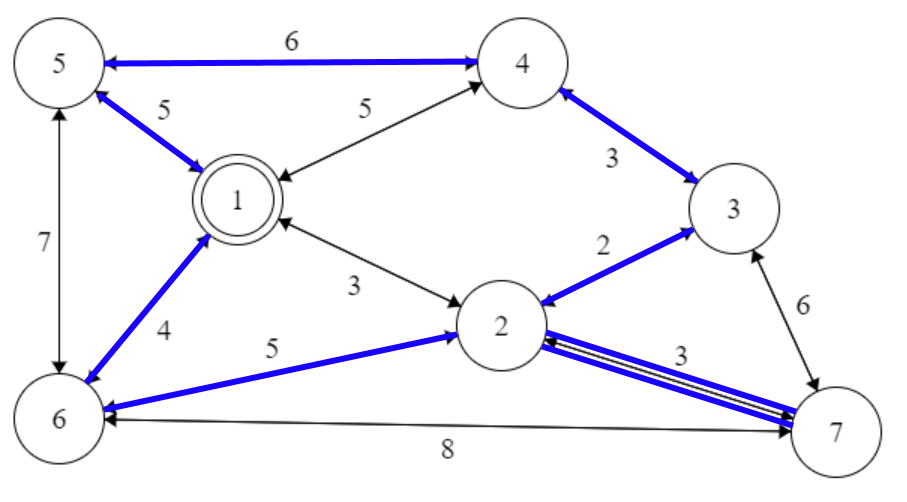
\includegraphics[width=0.9\linewidth]{../diagrams/tsp.png}
	\caption{Example of solved Traveling Salesman Problem where vertex 1 is the starting and ending node, and the bold path is the optimal path.}
	\label{TSP fig}
\end{figure}

\subsection{n Queens Problem}
This problem consists of finding a state of an \emph{n} x \emph{n} chessboard with \emph{n} queens such that no two queens threaten each other. The complexity here arises when you consider that in chess a queen can move horizontal, vertical, or diagonal any distance.

\begin{figure}[h]
	\centering
	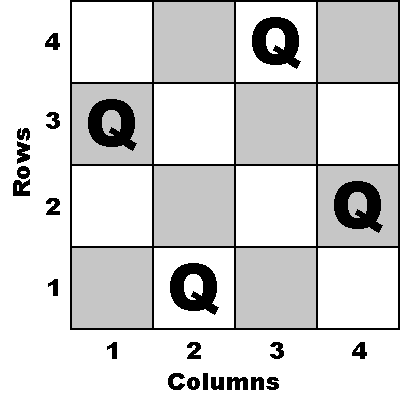
\includegraphics[width=0.7\linewidth]{../diagrams/nqueens.png}
	\caption{Example of solved 4 Queens problem.}
	\label{Nqueen fig}
\end{figure}

\subsection{Boolean Satisfiability Problem}
Given a boolean formula \emph{f} with considered variables \emph{V}, the Boolean Satisfiability Problem (SAT) is the problem of determining whether any state of \emph{V} satisfies \emph{f}. The SAT has been extended to many other problems due to its complex nature and due to the fact that it was the first problem proven to be NP-complete. One of the most notable problems is the 3SAT problem which contains a formula in conjuctive normal form \emph{f} containing \emph{n} clauses that are each limited to three variables \emph{x, y, z ${\in}$ V}.

\begin{figure}[h]
	\centering
	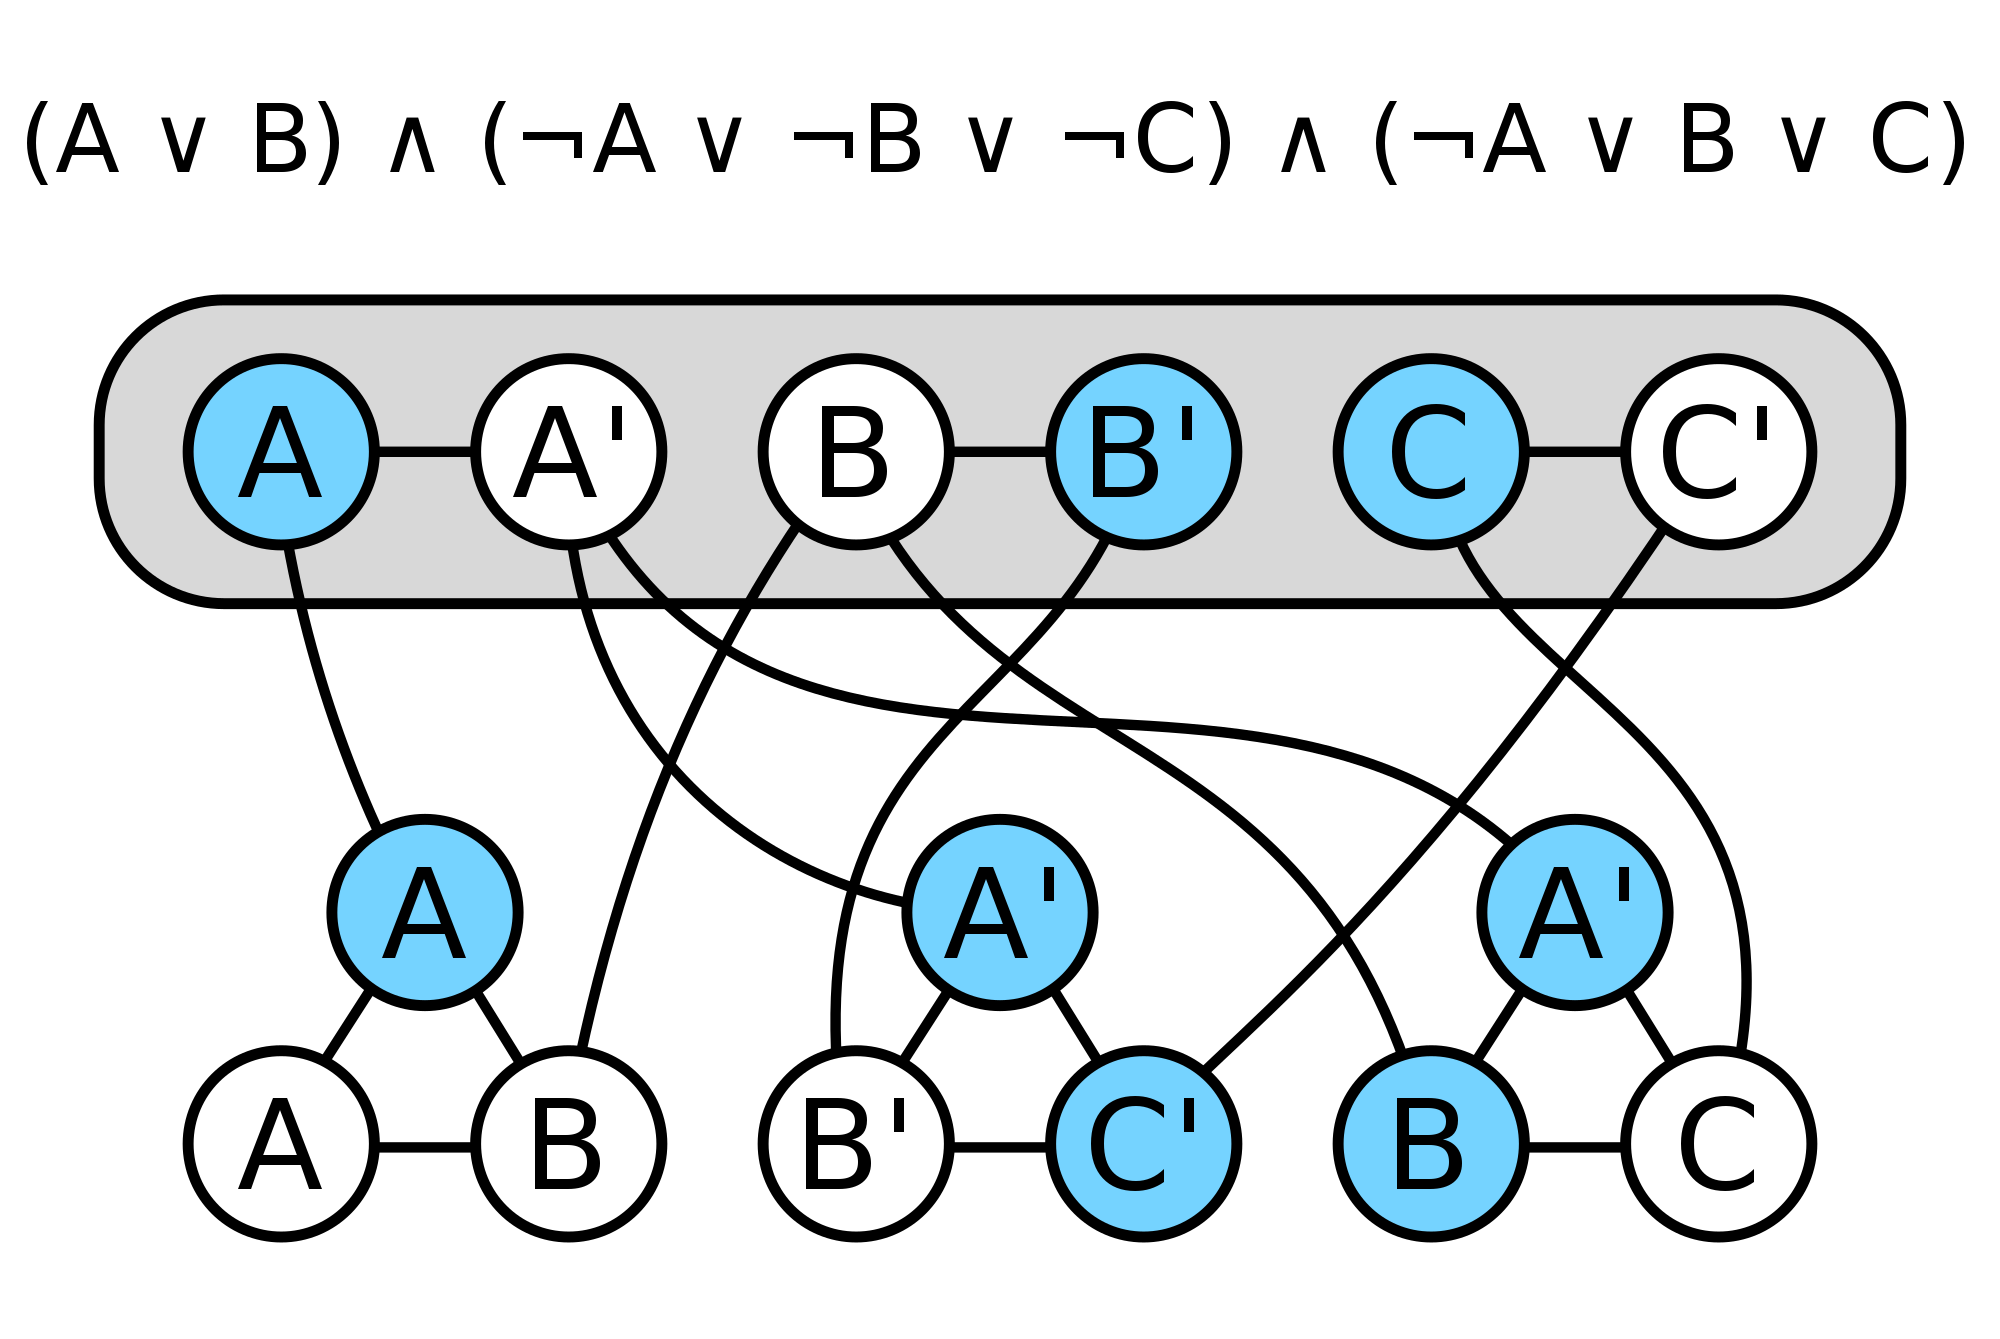
\includegraphics[width=0.7\linewidth]{../diagrams/3sat.png}
	\caption{Example of 3SAT. As long as each clause (triangular graphs) has a path leading to an accurate value (blue colored tuple element) this problem set is satisfiable.}
	\label{3SAT fig}
\end{figure}

\subsection{Job Shop Scheduling Problem}
Given \emph{n} jobs and \emph{m} processors, find a distribution of job assignment that results in all jobs being completed as quickly as possible. This is the job shop scheduling problem (JSP). This problem commonly arises in optimizing computer architecture and hardware, and is a common area of study when it comes to process parallelization.This problem can be altered to any sort of schedule conflicting problem.

\begin{figure}[h]
	\centering
	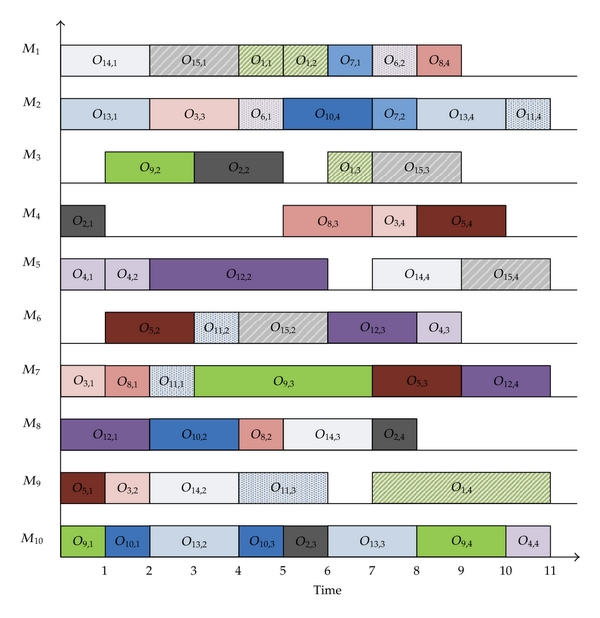
\includegraphics[width=0.7\linewidth]{../diagrams/jsp.jpg}
	\caption{$M_{x}$ is the machine. $O_{y,z}$ where $y$ is the job, and $z$ is the $z^{th}$ time this problem has been executed.}
	\label{JSS Fig}
\end{figure}

\subsection{Graph Coloring Problem}
Given constraints \emph{C} on a graph \emph{G = \{V, E\}}, the graph coloring problem (GCP) is to create an assignment of colors to vertices of the graph that meets the constraints in \emph{C}. Constraints are often similar to, ''Orange vertices may only connect via an edge to other orange vertices or blue vertices."

\begin{figure}[h]
	\centering
	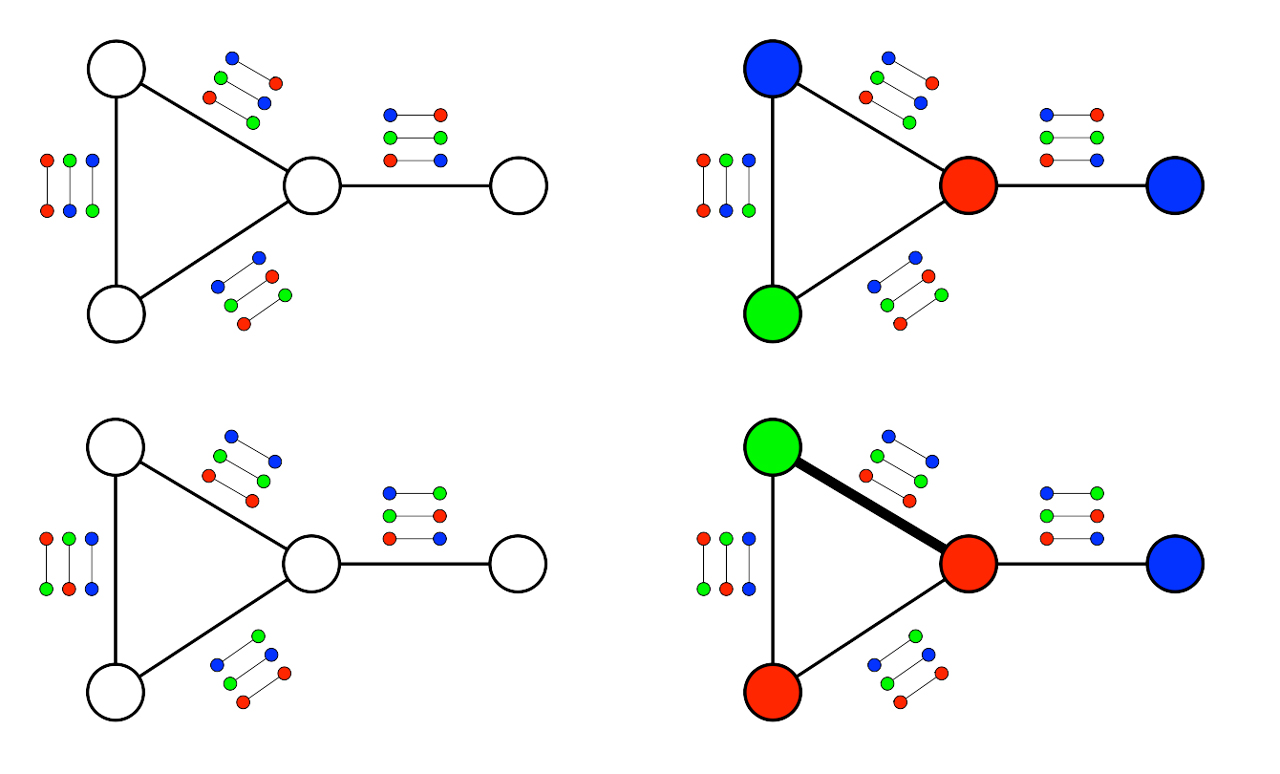
\includegraphics[width=0.7\linewidth]{../diagrams/GCP.jpg}
	\caption{Graphs that show the potential options of each edge to satisfy the constraints. The bottom right image demonstrates that certain constraints deem the problem impossible.}
	\label{GCP Fig}
\end{figure}

\section{Evaluation Metrics}
To evaluate our heuristic model we will compare a heuristic generated with our model against an algorithm with no heuristic (exhaustive) and against multiple state-of-the-art heuristics for the given problems. We will be comparing time complexity, space complexity, and accuracy to determine the effectiveness of our model. We will be testing on a single core of an Intel i5-6600k CPU @ 3.5GHz with 16gb RAM.

Time complexity will be measured in seconds, in which the lowest value is the most efficient.

Space complexity will be measured in number of vertices in the tree, in which the lowest value is the most efficient.

Accuracy will be measured by the percentage of correctness vs the most optimal solution, in which a value of 100\% is a perfect metric.

Ease of use will be measured by studying participants that use the model to create heuristics for various problems.

\section{Experiments} \label{Experiments}
To create a successful model, we must first determine what makes a good heuristic. Due to the intense level of research done in this area, we have multiple state-of-the-art heuristics to study and learn from.

We will start by implementing a generic CSP system written in C\# and accompany it with a BnB algorithm that operates based on a heuristic function. We will then verify the sanity of our system and algorithm by running the state-of-the-art heuristics and comparing results. Similarly, we will verify that the exhaustive method of having no heuristic provides the space complexity that can be mathematically calculated for each problem.

Once we have a working system that has proven to be accurate, we will create an algorithm for testing many iterations of heuristics. This will show us what traits of the problem become the most significant to discovering an effective model. Similarly, we will compare these results across all problems because our goal is to create a model that works across all CSPs.

To test the effectiveness of the model, we will inform a group of entry level computer scientists at the University of Colorado at Colorado Springs what the objective function of these algorithms are and have them develop a simple heuristic to optimize the task. Similarly, we will take this same group along with a secondary group of students that will be given the same objective but have them use our proposed model. We expect that students who use the model will create a much more effective heuristic than those who don't.

\section{Related Work}
Considering our goal is to create an effective heuristic model, a big element we need to consider is what makes a heuristic model great. Meta-heuristics are heuristics that are designed to select the proper heuristic for the given problem, or to generate a new heuristic if necessary. We will be playing the role of a meta-heuristic in this paper so understanding them is vital. D.F. Jones et al. \cite{JONES20021} surveys meta-heuristics for problems that have multiple objectives. This paper states that meta-heuristics are powerful considering they can handle integer variables, discrete variables, and/or logical variables which allows for application against many problems. Non-standard goals, constraints, objectives and conditions can be easily incorporated into a meta-heuristic which even further demonstrate their flexibility.

Bektas and Tolga \cite{bektas2006multiple} survey research on the multiple traveling salesman problem (mTSP). From this survey we get an understanding of the state-of-the-art algorithms that solve mTSP, and can directly apply them to other CSPs. The authors explicitly state, ``To the best of our knowledge, no efficient heuristic algorithms exist for the solution of large-scale mTSPs" but suggest that further research on the heuristics that are known to be successful for the solution of vehicle routing problem (VRP) would be a great place to start. This gives us direction and potential for growth with our model, as we can explore solutions for similar problems to improve our model.

Bell and Stevens \cite{bell2009survey} survey the n-queens problem in great depth, even going as far as discussing theorems and multiple sub-problems. By studying both the problem and sub-problems, it helps produce an overall understanding that will help in the creation of a heuristic design to optimize these problems.

%\section{Background Work}
%TODO

\section{Research Plan}
\subsection{Challenges}
Creating an effective heuristic is challenging in itself, therefore creating a heuristic model is also going to be a big endeavor. We face a problem where if we analyze too few problems and state-of-the-art algorithms we will develop a localized heuristic model for those specific problems. We want to encapsulate the entirety of the CSP area which is going to be difficult in itself, but also difficult to test. 

Similarly, we face a problem where developing a fully CSP encapsulating heuristic model might prove to be vague and ambiguous. Trying to create a clear and concise heuristic model that works for every CSP is going to be incredibly difficult. We might need to add addenda in order to more accurately describe the model.

One of the most difficult challenges is quantifying our evaluations when it comes to our measurement of ease of use. We don't have multiple copies of the same person to create control groups so we will need to measure this differently than the other quantifiable metrics. We will create four testing groups that each participate in two stages. Unassisted $\rightarrow$ unassisted, unassisted $\rightarrow$ assisted, assisted $\rightarrow$ unassisted, assisted $\rightarrow$ assisted. By studying four groups, we hope to be able to see and quantify improvement by groups using the model.

\subsection{Timeline}
The goal is to have this research ready and finished by mid April, 2019 with the possibility of extending out to the end of July, 2019. The following lays out the general plan and dates in which we want them to be completed.
\subsubsection{Phase 1}
The first phase of our research will consist of building the generic CSP system which will allow for easy implementation of any CSP. We will also be creating the BnB algorithm with a customizable heuristic function in which we can solve the CSP. Finally, we will be creating a testing suite that can run many iterations of the problem with different heuristic functions to determine patterns or anomalies in which we can use to help build our model.

After our system is complete, we will test it against state-of-the-art heuristics and see if we get comparable results. We will finalize phase 1 by providing data

\subsubsection{Phase 2}
This phase will focus primarily on research gathering and alternate testing using our testing suite to determine exactly what details of a heuristic function increase the optimality of our problems. More importantly, we will research why these details are the cause of the increase of optimality. Our method of research is as follows:
\begin{itemize}
	\item Test current model against TSP.
	\item Modify model to fit TSP.
	\item Test model against NQueens.
	\item Modify model to fit NQueens and prior.
	\item Test model against SAT.
	\item Modify model to fit SAT and prior.
	\item ...
	\item ...
\end{itemize}

We will be starting with the TSP due to the significant amount of research surrounding it.

Using our research, we will create the first draft of our heuristic model and test its effectiveness against each of the problems by comparing it against the state-of-the-art. We expect to receive comparable results vs the state-of-the-art at this point.
\subsubsection{Phase 3}
Finally, we will stress test our model to find out if it has any major defects. We will stress test by applying this model to many CSPs in the field to see how efficient the results are.

We will wrap up phase 3 by finalizing our model with all of the data and research we have obtained thus far.

\subsubsection{Phase 4}
The final phase will be for testing our model using groups of students at the University of Colorado at Colorado Springs as described in section \ref{Experiments}. These results will be published along with the model and any research applicable to the understanding and application of the model.

\section{Significance of Research}
The significance of this research consists of two main facts. The first is that operations research and artificial intelligence are two booming fields in computer science. CSPs are common problems throughout these fields and by optimizing these problems at their base will result in an overall performance increase across a vast amount of research pursuits. Similarly, this research can be applied to many other areas as it will show the generalities behind generating an effective heuristic. The second significance is that heuristic based algorithms are something that influence every day life. Combine it with machine learning and you get an algorithm that will recommend Netflix movies and shows that you are going to like. Put it in a video game to make the game seem more realistic, as it learns your behaviors to throw appropriate level challenges at you. So many real-world implementations not only worry about having an effective heuristic, but evolving that heuristic over time depending on the different circumstances. This research will focus primary on creating an effective model that can be used to create efficient heuristics. However, developers and researchers can apply this model to a dynamic system so that it can move towards a better heuristic more quickly. 

By focusing on a low level topic like this, we can create a model that allows researchers working at a higher level to focus more on their work as opposed to the smaller details.

\nocite{*}
\bibliographystyle{ieeetr}
\bibliography{mybib}

\end{document}
